% This part is to be filled by Lars

\begin{frame}{Nearest Neighbour}
  \begin{block}{Single Nearest Neighbour}
    \begin{enumerate}
      \item Start at a random node
      \item Check distances to all unvisited nodes
      \item Go to the one with the shortest distance
      \item \texttt{GOTO 2} until all nodes are visited
    \end{enumerate}
  \end{block}
  \pause
  \begin{block}{Nearest Neighbour}
    \begin{itemize}
      \item Do Single NN for every starting node
      \item Choose the best
    \end{itemize}
  \end{block}
\end{frame}

\begin{frame}{Nearest Neighbour (cont.)}
      \begin{block}{Single Threaded}
      \footnotesize\inputminted[xleftmargin=1em,fontsize=\large,linenos]{rust}{./assets/03_NN_single.rs}
      \end{block}
\end{frame}

\begin{frame}{Nearest Neighbour (cont.)}
      \begin{block}{Multi Threaded}
        \footnotesize\inputminted[xleftmargin=1em,fontsize=\large,linenos]{rust}{./assets/03_NN_parallel.rs}
      \end{block}
\end{frame}


\begin{frame}{Benchmarks}
  \vspace{-0.25cm}
  \begin{figure}
    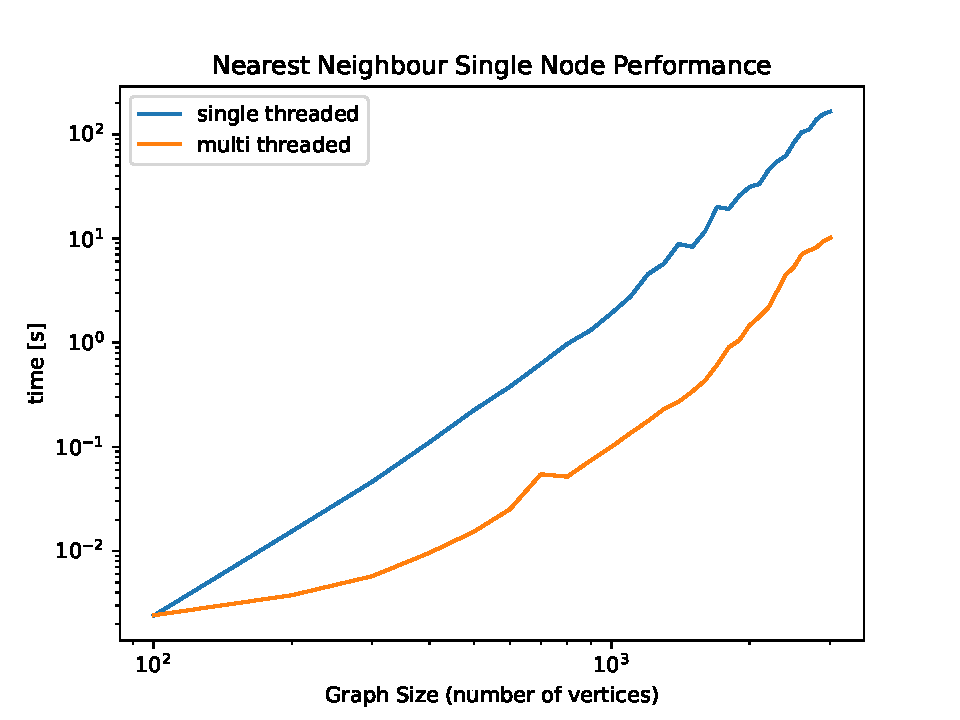
\includegraphics[width=\linewidth,height=.9\textheight,keepaspectratio]{../assets/nn-stmt.pdf}
  \end{figure}
\end{frame}

\begin{frame}{Nearest Neighbour: MPI}
  \begin{itemize}
    \item Divide number of nodes into equal chunks
      \pause
    \item Every process computes their chunks
      \pause
    \item \texttt{MPI\_Allreduce} the \textbf{cost} (and keep rank)
      \pause
    \item Winner rank \texttt{MPI\_Bcast} the solution path.
  \end{itemize}
\end{frame}

\begin{frame}{Benchmarks}
  \vspace{-0.25cm}
  \begin{figure}
    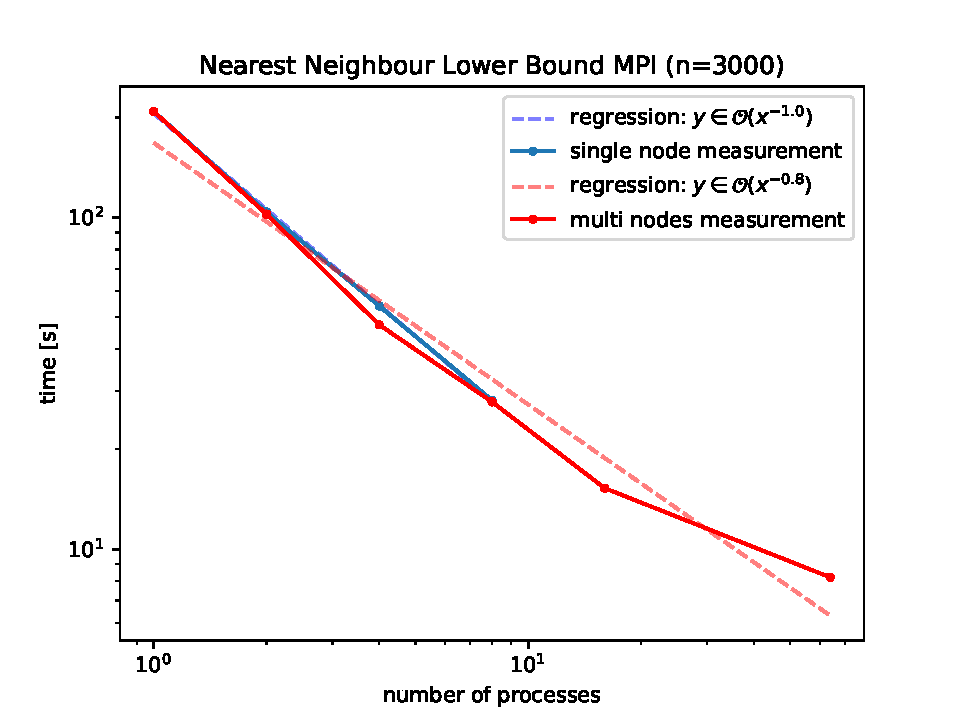
\includegraphics[width=\linewidth,height=.9\textheight,keepaspectratio]{../assets/nn-mpi.pdf}
  \end{figure}
\end{frame}
